\documentclass{article}
\usepackage[utf8]{inputenc}
\usepackage[english]{babel}
\usepackage{apacite}
\usepackage{graphicx}
\usepackage{mathptmx}
\usepackage{amsmath}
\usepackage{multirow}
\usepackage[font = {small, it}]{caption}
\DeclareCaptionLabelFormat{cont}{#1~#2\alph{ContinuedFloat}}
\captionsetup[ContinuedFloat]{labelformat=cont}
%\usepackage{subcaption}
\usepackage{subfigure}
\usepackage{float}
\usepackage{fancyhdr}
\usepackage{listings}
\usepackage{mathtools, nccmath}

\DeclarePairedDelimiter{\nint}\lfloor\rceil
\DeclarePairedDelimiter{\abs}\lvert\rvert

\lstset{language=Python}

%% CHANGE MARGINS

\addtolength{\oddsidemargin}{-.875in}
\addtolength{\evensidemargin}{-.875in}
\addtolength{\textwidth}{1.75in}

\addtolength{\topmargin}{-.875in}
\addtolength{\textheight}{1.75in}

%% make header

\fancypagestyle{plain}{
\fancyhf{}
\rhead{Mikkel Werling (201706722)}
\lhead{Unfriending facilitates cooperation}
\cfoot{\thepage}
}
\pagestyle{plain}

\setlength{\parindent}{2em}
\setlength{\parskip}{1em}
\renewcommand{\baselinestretch}{1.5}

\title{Unfriending facilitates cooperation: \\Co-evolution of opinion and network dynamics}
\author{Mikkel Werling, (201706722)}
\date{}
\begin{document}
\maketitle
\tableofcontents

\section{Introduction}

\subsection{Polarization, echo chambers and the threat to democracy}

Democracies around the world are experiencing increased amounts of polarization \cite{boxell_cross-country_2020,mccoy_polarization_2018, somer_deja_2018}. As a result, making decisions by cooperating with other people becomes harder which can severely damage the ability of democratic systems to solve problems \cite{andris_rise_2015,levin_dynamics_2021,mccoy_polarization_2018}. A striking recent example is uniquely severe rise of polarization of the political system in the United States \cite{dimock_america_2020}. During the last two decades, the amount of overlap of opinions between the two political parties have decreased substantially, which has led to gridlock, government shutdowns and failure to enact new legislation \cite{andris_rise_2015, pew_research_center_political_2014-1}. A similar increase can be observed in terms of affective polarization. Affective polarization refers to how much citizens carry more negative feelings towards other political parties than their own \cite{boxell_cross-country_2020, iyengar_origins_2019}. Once again, the United States is reported to have uniquely high amounts of affective polarization \cite{boxell_cross-country_2020}. Although the United States is unique in the extent of affective polarization, they are not the only country experiencing an increase in affective polarization. Countries such as France, Switzerland and Denmark has seen increased levels of affective polarization in the last two decades \cite{boxell_cross-country_2020}. Polarization is in other words a general trend, affecting countries around the world \cite{mccoy_polarization_2018, somer_deja_2018, wilson_polarization_2020}. With that said, a polarization of opinions does not seem to be an inevitable state for democracies. During the last two decades, a number of European democracies have experienced higher degrees of consensus and less affective polarization, which includes Sweden, Norway and Germany \cite{boxell_cross-country_2020}. 

There is reason to believe that the problem of polarization might be getting worse due to technology. Filters of what information is being given to us can create situations where almost all opinions one is exposed to are congruent with one’s believe, popularized under the term echo chambers on social media \cite{baumann_modeling_2020, sasahara_social_2021, tsai_echo_2020}. Relatedly, higher involvement in one’s echo chamber correlates with more negative emotions in terms of valence, which suggests that echo chambers are largely driven by outrage \cite{del_vicario_echo_2016}. With regards to polarization, the internet can be seen as a “mixed blessing” – it can drive opinions closer together by diversifying information, but it also enables encounters of opposing opinions by chance, which can increase polarization \cite{lev-on_happy_2009}. It therefore seems that there is a tension at play in how much exposure to different opinions affects polarization. When presented with diversifying views, people generally decrease negative affects to other political parties \cite{levy_social_2021}, but exposure to opposing views can cause opinions to become more polarized \cite{bail_exposure_2018}. 

Although polarization is usually referred to as a political phenomenon, polarization is important for any social system in order to cooperate successfully. It is therefore important that we understand what mechanisms can lead a system to polarization, to consensus or anywhere in between the two extremes. This is no easy task, as opinion formation is a highly complex phenomena \cite{baumann_modeling_2021}. Nevertheless, there is a rich history of research on the topic of opinion dynamics using experimental data in combination with formal models \cite{baumann_modeling_2021,chacoma_opinion_2015,flache_models_2017,friedkin_social_1990,noorazar_classical_2020,spears_social_2021,turner_paths_2018}. These models normally focus on mechanisms of social influence, where interactions between agents shape the agents’ opinions over time \cite{flache_models_2017}. Of special interest to this paper, the models typically assume a static network structure in which agents are situated \cite{galesic_integrating_2021}. This fails to take into account that networks are dynamic and co-evolves with opinions \cite{ferraz_de_arruda_modelling_2022,galesic_integrating_2021}. The interdependence between the dynamics of social networks and opinion dynamics is largely understudied, despite the fact that the two processes seem to influence each other in important ways \cite{asikainen_cumulative_2020,bruch_agent-based_2015,galesic_integrating_2021,kossinets_origins_2009,noorazar_classical_2020}. The dynamic relation between the network structure and social influence has often been reported as an important avenue for future research \cite{flache_models_2017,galesic_integrating_2021}. Additionally, the field is struggling to integrate empirical data in their models, which often leads to models that are not evaluated in terms of how well they correspond to the real world \cite{flache_models_2017,galesic_integrating_2021}. If we want to get closer to the answers of how opinions are formed in social networks, we need to make better use of the empirical data available as well as evaluate how well our models can explain the observed patterns of opinionated social networks. 

This paper seeks to investigating the co-evolution of the dynamics of opinions and networks by combining simple models based on insights from cognitive science, social psychology, computational biology and network science \cite{asikainen_cumulative_2020,flache_models_2017,ilany_social_2016,jackson_meeting_2007,santos_cooperation_2006}. This paper seeks to start filling the gap in the literature concerning the interconnected dynamics of networks and opinions. To do so, this paper attempts to estimate quantitatively how well the proposed network formation models fit empirical social networks. This paper investigates whether co-evolutionary models can better explain how social networks are formed. This leads to the central question that this paper will try to provide answers to. Namely, this paper’s central interest is to investigate what the effect of tie-deletion to dissimilar others has on facilitating cooperation. 


\section{Motivation of the framework}
\subsection{Agent-based models of complex issues}

In order to get sufficiently good answers to our questions, we need to build sufficiently good models. When it comes to models of opinion dynamics, this is no easy task. The social systems underlying opinion dynamics are complex and complicated. The change of opinions is both a cognitive matter of updating one’s belief, but also a social matter of being exposed to different perspectives \cite{flache_models_2017,friedkin_social_1990,spears_social_2021}. Models that do incorporate realistic social and cognitive mechanisms are typically verbal models. Although these accounts often provide rich and detailed realism, they lack the precision of formal models \cite{fogarty_ten_2022,galesic_integrating_2021,smaldino_how_2020}. Agent-based models are well-equipped to strike a balance between the two types of models \cite{flache_between_2018,galesic_integrating_2021,epstein1999agent,mas2014cultural} . This is done by investigating the macro-behaviors of a system, where the micro-behaviors are specified \cite{bruch_agent-based_2015,epstein1999agent,flache_between_2018}. As is the case with any model, the results critically hinge on the assumptions of the model. It is therefore the role of the modeler to provide as empirically plausible mechanisms as possible for the system of study \cite{crooks2012introduction,epstein1999agent,page2010diversity}. At the same time, the value of a model is in its simplification of reality. The model should be as simple as it can be and as complicated as it needs to be in order to answer the questions of interest \cite{smaldino_how_2020}. The hope is that by simplifying the system to a sufficient extent, we can observe and understand some important features of even extremely complex systems \cite{fogarty_ten_2022,smaldino_how_2020}. The modeler’s job is to strike this balance between realism and simplicity by including only the most central mechanisms of the system in their model \cite{smaldino_models_2016}. 

To incorporate these mechanisms in the model of this paper, we turn to identifying key aspects of how social interactions shape opinions and how networks change over time. We start by considering key features of social interactions. Here, we will focus on homophily as well as positive and negative social influence. Thereafter, we turn to network dynamics and discuss the central role of triadic closure in how networks are shaped over time.

\section{Central Mechanisms}
\subsection{Homophily}
One of the most robust findings of the social world is summed up in the now famous phrase "birds of a feather flock together" \cite{mcpherson_birds_2001}. This phrase refers to the fact assortativity in humans is non-random, and is often based on similarity \cite{asikainen_cumulative_2020,crandall_feedback_2008,mcpherson_birds_2001}. You are more likely to engage with other individuals that are similar to you \cite{taylor_exploring_2018}. This is true for almost all demographic variables which have been investigated, which includes gender, race, religion, and socioeconomic class \cite{asikainen_cumulative_2020,mcpherson_birds_2001}. In other words, people choose their friends in part to be reflections of their own traits and personality. 
Intuitively, it seems reasonable to assume that you have more in common with your friends than you have with strangers. To test this notion, Kossinets \& Watts (2009) recorded social interactions on a large university over the course of a year. Their findings not only suggests that this intuitive notion is true, but that it is a special case of a more general phenomenon. The findings suggests that distance in similarity is a function of distance in the social network (see Fig 1). The further you are removed from someone in the social network, the less you will have in common \cite{kossinets_origins_2009}. This seems to be a robust finding of social networks \cite{bener_empirical_2016,crandall_feedback_2008}, and has been explained by the two central dynamics that this paper focuses on. Namely, people are similar to the people they are connected to, because social influence makes them even more similar and that selecting new friends is largely based on similarity \cite{crandall_feedback_2008}. 

\subsubsection{Explaining Homophily}
Homophily is traditionally explained as a psychological preference for similar people \cite{asikainen_cumulative_2020,mcpherson_birds_2001,winter_you_2020}. Interacting primarily with similar people ensures easier communication and enhances the individual’s ability to predict the other person’s behavior \cite{kossinets_origins_2009,winter_you_2020}. Assorting based on similarity might facilitate cooperation, because coordination between similar individuals is simpler and less costly for the individual \cite{winter_you_2020}. This psychological explanation of the homophilic preference of individuals seems sufficient to explain the phenomenon of homophily, but structural constraints could also limit how dissimilar choices of interactions are available to a person \cite{peixoto_disentangling_2022}. If you work as a female nurse, chances are that most of your interactions at work will be with other females. In this case, even if you do not have a strong psychological preference for interacting with people like yourself, the social interactions available to you might primarily be people like yourself. Therefore, most of your interactions will be homophilic in nature because of existing assortment in the network based on similarity \cite{peixoto_disentangling_2022}. These structural constrains are of course not exclusive to gender or workplaces. Other examples include socio-economic status and the neighborhood you live in and preference in music and what concerts you attend \cite{mcpherson_birds_2001}. In other words, the psychological and the structural factor contributing to observed homophilic interactions are not mutually exclusive but might instead facilitate each other \cite{asikainen_cumulative_2020}. Even a little psychological homophilic preference could turn into structural factors over the course of time \cite{asikainen_cumulative_2020,kossinets_origins_2009,taylor_exploring_2018}. Empirical work points to both psychological and structural homophily being important mechanisms, but suggests that structural homophily might be a more powerful mechanism for finding new connections in a social network \cite{bener_empirical_2016,kossinets_origins_2009}.
As mentioned, the observed general finding of assortment in networks are not only based on selecting friends based on similarity. It is also due to the fact that humans interact with their social ties, which typically increases similarity (Friedkin \& Johnsen, 1990; Spears, 2021). The combined mechanism of social interactions in shaping opinions is called social influence and is what we turn our attention to next. 

\subsection{Social Influence}
Humans are inherently a social species. We think and form our opinions by discussing them with other people. 
Either via social media, debates or discussions with friends, opinions are constantly being shared between individuals. 
As a result of these social interactions, the opinions of people involved in the interaction might change. 
This process is normally referred to as social influence and has been proposed as the most important effect in shaping an individual’s opinions \cite{chacoma_opinion_2015}. 
In this paper, we will distinguish between positive and negative social influence. Positive social influence refers to interactions that result in more similarity between agents after interacting \cite{flache_models_2017,levin_dynamics_2021}. 
This can be thought of as reaching a compromise, finding common ground or seeing the other person’s perspective on a topic. Negative social influence refers to interactions that result in less similarity between agents after interacting \cite{flache_models_2017}. 
Examples include moral outrage, outgroup aversion or similar distancing effects. It is important to note that although positive influence seems to be a robust empirical finding, negative influence is more elusive \cite{flache_models_2017,takacs_is_2014,turner_paths_2018}. 
With that said, there is evidence that suggests that exposure to opposing views can lead to increased polarization \cite{bail_exposure_2018}.

\section{Opinion Dynamics}
The effects of homophily and social influence has been studied extensively with different types of formal models, primarily agent-based models \cite{flache_models_2017,flache_between_2018,noorazar_classical_2020}. These simplified systems are normally studied to identify which conditions can give rise to polarization or consensus in terms of the opinions of simulated agents \cite{flache_models_2017}. Previous models have largely only focused on how social influence affects a system over time, without considering how the social interactions change as a result of changes in opinions \cite{galesic_integrating_2021,holme_nonequilibrium_2006,jalili_coevolution_2015}. Central to most classical models of opinion dynamics is that agents are situated in static, theoretical networks \cite{flache_models_2017}. The assumption of static networks is not inconsequential. Social networks are inherently dynamic, with new ties being formed and deleted over time.  But as has already been established, empirical work suggests that these two processes are largely interdependent \cite{bener_empirical_2016,kossinets_origins_2009}. New social interactions are more likely between similar agents, and tie deletion is also more likely between dissimilar agents \cite{kossinets_origins_2009}. 
Although all models do some violence on the world by making assumptions, models should try to include the vital mechanisms of the system they are representing, while simplifying the system enough to understand it \cite{epstein1999agent,smaldino_models_2016}. Considering the empirical evidence \cite{bener_empirical_2016,crandall_feedback_2008,kossinets_origins_2009}, it is one of this paper’s central claims that coevolution should be considered a vital mechanism. Coevolution is largely understudied in current models \cite{flache_models_2017,galesic_integrating_2021,sasahara_social_2021}. It is therefore one of the central interests of this paper to throw away the assumption of static networks, and instead investigate the coevolution of opinions and social networks. To achieve this, we need to expand our understanding of the basic underlying mechanisms of social influence to also incorporate the underlying mechanisms of network formation. We therefore turn our attention to identifying empirically plausible micro-behaviors of network formation. 

\section{Network Formation}
In order to identify realistic mechanisms of network behavior, it is fruitful to first survey previously considered networks in opinion dynamics. 
Classic examples of the static, theoretical networks used in most models include ring lattices, small-world networks and scale-free networks \cite{barabasi_scale-free_2003,watts_collective_1998}. Both small-world and scale-free networks are famous for being able to capture essential features of real social networks. Namely, small-world networks are able to capture the general tendency of large average clustering coefficient and small average path length \cite{watts_collective_1998}. Famously, this is achieved by starting with a ring lattice and rewiring a small percentage of the ties randomly, which creates highways of information that decreases the average path length considerably \cite{watts_collective_1998}. On the other hand, scale-free networks can capture the general tendency of long tails in degree distributions of social networks. That is, the degree distribution of social networks often follows a power law, where a few nodes have an extreme amount of edges, while most nodes only have a few \cite{barabasi_scale-free_2003}. Recent work seems to call into question how universal power laws are in empirical social networks, and finds instead that most networks follow a lognormal distribution, and not a power law \cite{broido_scale-free_2019}. It is noteworthy that neither of the theoretical networks can capture the essential features of social networks simultaneously \cite{jackson_search_2004}. As these features are likely to be critical to the behavior of how the agents interact in such a network, we need more empirically plausible models of social network formation. 
\subsection{Triadic Closure}
An alternative to the preferential attachment of scale-free networks and the rewiring of small-world networks is to consider what mechanisms govern how real social networks change over time. Both scale-free and small world networks attempt to answer the question of how networks characteristics could be generated, not why social networks have the characteristics that they do \cite{jackson_search_2004}. An attempt at answering the why-question is the work by Jackson \& Rogers (2004), which emphasizes the role of triadic closure in network generation. Reliably, triadic closure is found to be the most robust mechanism for how new connections are made in social networks \cite{asikainen_cumulative_2020,bianconi_triadic_2014,kossinets_origins_2009,peixoto_disentangling_2022}. Triadic closure refers to generating new connections by selecting from “friends of friends”. Empirical studies on dynamical networks find that the probability of creating a new tie is a decreasing function of the distance in the network \cite{bener_empirical_2016,kossinets_origins_2009}. The less separated you are from someone, the more likely you are to form a social tie to this person. Specifically, the empirical study suggests that when you are removed one rather than two degrees of separation from someone, you are 30 times more likely to form a connection. This increase in likelihood only increases with distance. When you are 5 degrees of separation away, you are 2.500 times less like to form a connection than you would have been were you only removed by one degree of separation \cite{kossinets_origins_2009}. 

Using triadic closure as the generating principle for network formation has shown great promise in explaining some of the key characteristics of social networks. In formal models, this is implemented by making new connections predominantly by triadic closure while letting a small percent of new ties be formed at random \cite{ilany_social_2016,jackson_search_2004,jackson_meeting_2007}. These models can generate the important characteristic findings of high average clustering coefficient, low average path length and lognormal degree distributions \cite{jackson_search_2004,jackson_meeting_2007}. 
It is worthwhile to take time to understand why these measures are important and why these models generate the patterns that they do. Average clustering coefficient is a measure of connected local communities are in the network \cite{watts_collective_1998}. Models of triadic closure are likely to exhibit high average clustering coefficients as triadic closure will increase the number of local links. This is closely linked to the fact that social networks are often made of tight-knitted, well-connected local communities \cite{peixoto_disentangling_2022}. Average path length refers to average length of the smallest path between any node in the network. Here, the implemented formal models of triadic closure benefit from similar mechanisms of randomness as small-world networks to achieve low average path lengths \cite{jackson_meeting_2007,watts_collective_1998}. Having even a small amount of randomness can create long-range connections, that acts like shortcuts between nodes, decreasing the average path length substantially \cite{watts_networks_1999}. Path length is important for how fast information or contagious diseases can spread between individuals in a network. Finally, triadic closure will lead to lognormal or scale free degree distributions, as high degree nodes have more possibilities for being selected for tie generation simply because they have larger degrees \cite{jackson_meeting_2007}. The principle of triadic closure seems to not only characterize human social networks, but could be a robust organizing principle for many different social species \cite{ilany_social_2016}. 

\section{Co-evolution via tie-deletion}
Now that we have established the fundamental principles of opinion and network dynamics, we now turn to the mechanisms that could enable them to co-evolve. As has already been proposed, each social agent is primarily being exposed to opinions by their peers. Therefore, the social network already influences opinion dynamics. Therefore, any mechanism that changes the ties in the network based on the opinions of the agents will cause opinion and network dynamics to co-evolve. There are good reasons to believe that such effects are abundant. Similarity is a strong predictor of which pairs form new ties \cite{bener_empirical_2016,kossinets_origins_2009}. In the same vein, dissimilarity also predicts the breaking of social ties \cite{bener_empirical_2016,kossinets_origins_2009,levin_dynamics_2021}. Although both mechanisms are at play in social networks, we will focus our efforts on tie-deletion of dissimilar ties. The reason for this choice is that there are already existing work focusing on the effects of tie-deletion in similar models \cite{santos_cooperation_2006,sasahara_social_2021}. This allows us to examine the robustness of the effect of tie-deletion on opinion dynamics. It is these papers that we now turn our attention to.  

\subsection{Tie-deletions effect on cooperation}
In addition to the empirical work investigating the interplay between social networks and the opinions of their constituents, theoretical work also points to the primacy of the co-evolution of networks \cite{holme_nonequilibrium_2006}. Specifically, the literature from an adjacent field of opinion dynamics, namely computational biology, suggests that co-evolution can play a vital role in facilitating cooperation \cite{dakin_dynamic_2018,melamed_strong_2016,pepper_mechanism_2002,santos_cooperation_2006}. Intuitively, one might expect that when connectivity increases in such a network, cooperation increases as well. However, the opposite effect is observed. In their paper, Santos et al. (2006) considers agents playing game-theoretic games, where agents either cooperate or defect. In relation to the mechanism of tie-deletion, Santos et al. (2006) proposes a way for agents to adjust their ties based on interactions made with other agents. When cooperators interact with defectors, the social tie between cooperators and defectors has a chance of being rewired to a different agent. This keeps the number of edges constant, but decreases connectivity \cite{santos_cooperation_2006}. Their results indicate that as the propensity for deleting ties between cooperators and defectors increases, cooperation flourishes. The more likely tie-deletion is, the more cooperation evolves in the system. The reason given for this result is that removing ties between cooperators and defectors increases positive assortment between cooperators and decreases positive assortment between defectors and cooperators. One of the striking attributes of this finding is that without any propensity for tie-removal, cooperation does not evolve for conditions equivalent to the Prisoner’s Dilemma \cite{santos_cooperation_2006}. More generally, positive assortment has been found to be a robust facilitator of cooperation in computational biology \cite{boyd_coordinated_2010,dakin_dynamic_2018,melamed_strong_2016,pepper_mechanism_2002}. The results also indicate that even relatively simple topological network dynamics that reflect the individual agent’s reaction to their social interactions can produce realistic networks \cite{santos_cooperation_2006}. 
Despite the generality of positive assortments effect on cooperation, work in the opinion dynamics literature points to an opposite result. When combined with social influence, they report that tie deletion can lead to echo chambers, that stifle cooperation \cite{sasahara_social_2021}. This is more in line with a more intuitive explanation, where a decrease in the communication between agents leads to a decrease in cooperation. Moreover, this work also Obviously, computational biology and opinion dynamics are not same field, but it is still noticeable that the same underlying mechanism gives rise to effects of opposite directions on a networks ability to cooperate. Both studies are interested in how the dynamics of the network influences how well agents cooperate in the network, and they both find that tie-deletion is critical to developing cooperation \cite{santos_cooperation_2006,sasahara_social_2021}. It is precisely because of this dispute that this paper is especially interested in how the deletion of negative ties can impact cooperation. Like the work of Santos et al. (2006), the probability of deleting negative ties will therefore be a key aspect of our model.  


\section{Model Description}
\subsection{Conceptual overview}
The model consists of agents situated in an undirected network. Nodes on the network represent social agents. Edges represent social ties to other agents. 
The model simulates social interactions between the agents without agents having any strategy or task. 

\subsection{Assumptions}
It is assumed that the opinion of an agent is shaped only by her initial opinion and the influence of her peers. 
The model assumes that agents will compromise their opinion when interacting with agents with similar opinions. 
When agents interact with agents dissimilar from them, the model assumes that agents will either not change their opinion or they will become more opposed by the interactions.
Furthermore, it is assumed that connections between agents are not static but dynamic in nature. 
Specifically, the model assumes that agents will find new connections primarily through their already existing connections. In other words, 
agents primarily find new friends via "friends of friends". Finally, it is assumed that agents will tend to relinguish ties to agents too dissimilar from themselves.
All these assumptions can vary in the strength of the proposed effect. For instance, similar agents could reach a perfect compromise or only convince each other slightly. 
As the results of the model critically hinges on the strength of these assumptions, I introduce model parameters that control the strength of these mechanisms.


\subsection{Components and their properties}
The model is specified by four different parameters. 
The first three describe how interactions change opinions ($\alpha$, $\beta$, $T$). 
The fourth parameter specifies the probability of dissoluting negative ties ($D$).
The specifics of how they influence the model is specified in "Dynamics".  

To limit the combinations of different values, we limit the possible values of the different parameters with the following:


\begin{align*}
    \alpha \in & \{0.05, 0.10, 0.15, 0.20, 0.25\} \\
    \beta \in & \{0.00, 0.05, 0.10, 0.15, 0.20, 0.25\}\\
    T \in & \{0.8, 0.9, 1.0, 1.1, 1.2\}\\
    D \in & \{0.0, 0.2, 0.4, 0.6, 0.8, 1.0\}
\end{align*}


\subsection{Initialization}
A random Watts-Strogatz small-world graph is created 
with $N=500$, $k=7$, and $p=0.5$. For each node in the network,
an agent is initialized with a value ($O_i$) which is taken to represent the opinion of the agent. The opinion is modelled as a continous number between -1 and 1. 
The idea is to represent that opinions can be anywhere inbetween extremely pro and extremely against a proposition.
To initialize the model, we start of with a diverse set of opinions. All values of $O_i$ are initialized by drawing from a uniform distribution between -1 and 1: 
$$O_i \sim U(-1, 1)$$

\subsection{Dynamics}

\subsubsection{Sampling agents and interactions}

The model is an attempt at representing social encounters and their change over time. 
To represent this idea, agents interact with each other over a certain amount of time-steps. 
During such a time-step, an agent will encounter a new connection. 
At every timestep ($t$) a random agent ($A_t$) is sampled from the network ($N_t$). This agent creates a new edge to another agent in the network. The network occationally deletes edges.
To keep the number of edges in the network approximately constant, edges are either created or rewired to account for deleted edges. 
To do this, let $E_1$ be the number of edges of $N_1$ and let $E_t$ be the number of edges of $N_t$. 
If $E_t < E_1$, $A_t$ will not rewire one of its existing edges, but instead create a new edge. If $E_t \geq E_1$, $A_t$ will rewire one of its existing connections to the new agents.
With a probability of $R$, $A_t$ connects to a random agent, that $A_t$ is not currently connected to. 
With a probability of $1-R$, $A_t$ connects to one of its edge's edges. Regardless of whether the connection was sampled randomly or through an edge's edges, let $C_t$ define the newly connected agent.
In the rest of the paper, we will only consider $R=0.1$. The reason for this is that this shows very little effect on the overall results, and low randomness is in line with empirical findings on the tie formation.

In order to calculate the average path length of the network, the model is restricted to being only one component. 
To ensure this property, we check the degree of $A_t$ and $C_t$. If the degree of either $A_t$ or $C_t$ is 0, a new edge is created randomly to a new node from $N_t$.
If both $A_t$ and $C_t$ have degrees larger than 0, and the network has more than one component, a new edge is created to restore the network. Specifically, we restore the edge that $A_t$ rewired to $C_t$, while keeping the edge from $A_t$ to $C_t$.
I will refer to the process of ensuring only one connected component simply as component ensurance. 

\subsubsection{Interaction between neighbors}
After finding a new connection, the agents interact with each other. This is meant to represent 
discussion, statements or other social interactions between agents. 
Social interactions between similar individuals will lead to compromise between their initial opinion and their opinion after the encounter.
As a consequence, the more you disagree with a person, the more mallable your opinion is. If you reach a compromise with a person with a very different opinion than yours,
you will change your opinion more dramatically than if you reached a compromise with someone that you almost agree with. 
To model this kind of behavior, the randomly sampled agent, $A_t$, interacts with all its connected agents and changes its opinions according to the opinion of the connected agents.
This is done by iteratively interacting with every edge of $A_t$. Let $B$ denote an edge of $A_t$. Let $O(\cdot)$ define a function with agents as inputs and their opinions as outputs.
The interaction between two different agents is determined by a threshold value, $T$. 

When $T \geq \abs{O(A_t) - O(B)}$, the interaction will pull the opinions of the two agents closer to each other. The force with which they are pulled is defined as a fraction of their distance from each other:
$$V_p = \big(\abs{O(A_t) - O(B)}\big) \cdot \frac{\alpha}{2}$$

Let $O_{max} = \max(O(A_t), O(B))$ and $O_{min} = \min(O(A_t), O(B))$ and update the values of opinions by:

$$O_{max} = O_{max} - V_p$$
$$O_{min} = O_{min} + V_p$$

When $T < \abs{O(A_t) - O(B)}$, the interaction will push the opinions of the two agents further apart by a similar principle as illustrated above: 

$$V_n = \big(\abs{O(A_t) - O(B)}\big) \cdot \frac{\beta}{2}$$

Using the same definition for $O_{max}$ and $O_{min}$, we update the opinions of each agent:

$$O_{max} = O_{max} + V_n$$
$$O_{min} = O_{min} - V_n$$

This process concludes when $A_t$ has updated her values for all her edges.

\subsubsection{Tie-dissolution}
After interacting with her connected agents, $A_t$ might delete the connection to some of these agents based on their similarity.
In this model, social interactions can result in opinions becoming more distant than they were initially. 
This can be because what the agents are discussing is divisive or controversial. When this happens, connections can be severed.
I call this process tie-dissolution. 
If $T < \abs{O(A_t) - O(B)}$, there is a chance that their tie is dissoluted after interacting. This probability of dissolution between dissimilar agents in the model is described by the parameter $D$.
When $D = 1$, all dissimilar ties are severed. When $D = 0.5$, there is 50\% chance that dissimilar ties will be deleted. 
After ties are dissoluted, the process of component ensurance is performed where $C_t$ is replaced with $B$.
When all edges of $A_t$ have been evaluated, the time-step concludes. This process is repeated for 10.000 time-steps.

\subsection{Outcome metrics} 

\subsubsection{Time-dependent Metrics}
Every 20th time-step, the current state of the network is recorded. 
To track the polarization of opinions over time,
the mean and standard deviation of the absolute value of opinions are recorded.
To track the similarity of an agent's opinion to the opinion of their neighors, the average distance to all edges are recorded.
To evaluate the effect of tie-dissolution, the cumulative frequency of tie-dissolutions are recorded.
For characterizing the network, I record the average clustering coefficient, average path length and degree assortativity coefficient.

\subsubsection{Final State Metrics}
After 10.000 time-steps, the network reaches its final state and its characteristics are recorded. 
For every agent in the network, I record: 
\begin{itemize}
    \item The initial opinion of the agent
    \item The opinion of the agent at the final state of the network
    \item The mean distance to all neighbors' opinions
    \item The degree of the agent 
    \item The betweeness centrality of the agent 
    \item The clustering coefficient of the agent 
\end{itemize}

The measures related to the opinion of agents can then be correlated with clustering, centrality and degrees to see how changes in network topology relate to changes in opinions. 

\section{Model Evaluation}

\subsection{Fitting the model}
As previously mentioned, previous models have often not integrated empirical data of social networks sufficiently to test the validity of their models (Flache et al., 2017). What is meant by this critique? Arguably, the most pressing issue is that models rarely consider how the results of their computational models compare with the real world. This is largely a product of the types of agent-based models typical in opinion dynamics as well as the phenomena of opinion dynamics themselves. Most models of opinion dynamics are low-dimensional (Bener et al., 2016), in that they don’t seek to explain exhaustively how opinions are formed, but rather to point out interesting interactions between key variables of the process. This makes empirical validation especially tricky for these models. Compounding to this problem is that the time-scales considered by these models are massive, and that kind of data is very hard to come by. And even if they were available to us, opinions are very hard to measure. Any self-reported measure is going to be subject to the usual problems of the unreliability of self-reports. Using political voting patterns might be a usable proxy for polarization, but these data are very hard to come by. 
This does not however mean that incorporation of empirical data is impossible. Because the model considered in this paper is coevolutionary, it allows us to investigate how the generated networks compare to real empirical social networks. By borrowing methodology from computer science, we will treat this as a machine learning problem, and investigating the goodness of fit using hyperparameter optimization (Akiba et al., 2019; Bergstra et al., 2011). What we really want to know is to what degree the model can explain the patterns observed in real world social networks. To do this, we want to estimate the model parameters by generating networks from the model, and then see how much these generated networks resemble real networks. I will refer to the process of finding these parameter values as agent-based model fitting, as it is analogous to estimation of parameter values in statistics. Beyond knowing whether the model can generate the observed structure of real-world networks, this paper is specifically interested in how critical co-evolution is to the explanatory power of these models. Ideally, we want to compare models which include co-evolution to models without co-evolution and investigate whether co-evolutionary models are better explanations than their network formation counterparts. I will refer to this process as agent-based model comparison, which is again reasoned by its analogy to model comparison in statistics. 
Although these steps are analogous to model fitting and model comparison, there are important differences that are worth mentioning. Especially important is that model comparison normally penalizes the inclusion of additional parameters in the model (Vrieze, 2012). In other words, simple explanations are preferred when the performance is comparable (Emiliano et al., 2014; Vrieze, 2012). The primary reason for this is that including additional parameters allows the model to overfit to the data. In classical regression models, models with additional parameters will always give a better fit, as the scalar for the new parameter can simply be set very close to zero. In this case, the model becomes mathematically identical to the simpler explanation. Although we don’t have a formal way of calculating agent-based equivalents to Akaike Information Criteria or Bayesian Information Criteria to determine which model is the better explanation (Vrieze, 2012), we can try to avoid situations of mathematical identity and overfitting. This is done by framing the problem of agent-based model fitting as a hyper parameter optimization problem. 


\subsection{Data}
To fit the model to data, we consider 6 empirical social networks; a network of representing social networks of Dolphins (Lusseau, 2003), the Karate Club Network (Zachary, 1977), a citation network (Newman, 2006), co-purchase network of political books on Amazon (Shi et al., 2017), political blogs (Adamic \& Glance, 2005) and network of politicians based on shared likes on Facebook (Rozemberczki et al., 2018). For all networks, only the main component of the network was considered. This was done as average path length is not well-defined for unconnected graphs. As the model assumes undirected networks, the network of political blogs was transformed from a directed to an undirected network. This was done by making any directed link between two agents be undirected. 

\subsection{Hyperparameter Optimization}
To evaluate how closely the generated networks resemble the real networks, we must first define a distance metric between networks. Although many features are important for characterizing a network, we will follow previous suggestions that identify the average path length, the average clustering coefficient and the degree distribution as the most defining aspects of a network (Jackson \& Rogers, 2004, 2007). We therefore seek to minimize the mean difference on these parameters between the generated and the real networks. 
Before we can simply calculate the mean of difference, there are some specifics that needs to be clarified. These primarily concern the average path length and how to operationalize the difference in degree distributions. 
To identify the distance of degree distributions of networks, we calculate the Jensen Shannon Divergence between the two distributions. The Jensen Shannon Divergence is a distance metric between probability distributions \cite{fuglede_jensen-shannon_2004}. 
In terms of the average path length, there is a problem of computational costs. Calculating the average path length can be very expensive computationally, especially for large networks (Matsumura et al., 2018). Instead of calculating the actual average path length, we approximate it by taking 1000 samples of random pairs of nodes and calculating the average path length of those 1000 nodes. Although this is still only an estimation of the actual average path length, this method generally approximates the average path length fairly well (Matsumura et al., 2018).
Both the correlation coefficient and the Jensen Shannon Divergence are values between 0 and 1. Average path length on the other hand is not restricted in the same way. If it is not normalized, it will therefore be weighted much higher than the correlation coefficient and the Jensen Shannon Divergence in the distance metric. We therefore normalize the average path length by

$$APL* = \frac{\abs{APL(G) - APL(A)}}{APL(A)+2}$$

where $APL*$ is the normalized average path length, $APL(G)$ is the approximated average path length of the generated network and $APL(A)$ is the apprioximated average path length for the actual network. Adding two to the denominator is somewhat arbitrary. The choice was made to be more certain that $APL*$ would still be below 1.
With this in place, the final distance metric considered between the actual network, $A$ and the generated network $G$ is 

$$ O(A, G) = \frac{1}{3} \cdot \left(JSD(D(A), D(G)) + \abs{C(A) - C(G)} + APL*\right)$$

where $O(A, G)$ is the distance between distance between the two networks, $JSD$ is the Jensen Shannon Divergence, $D(A)$ is the degree distribution of $A$, $D(G)$ is the degree distibution of $G$, $C(A)$ is the average clustering coefficient of $A$ and $C(G)$ is the average clustering coefficient of $G$. This distance metric is just the average difference on the considered network characteristics between $A$ and $G$. This is also why the sum of the difference is multiplied by $\frac{1}{3}$. This distance metric between networks, $O(A, G)$ will serve as the objective function that we want to minimize. The hyperparameter optimization algorithm search the parameter space for the combination of parameters that results in the lowest values of $O(A, G)$ \cite{akiba_optuna_2019,wu_hyperparameter_2019}.

All models were fit by first calculating the ratio between edges, $E$, and vertices, $V$, and calculating $K = \nint{(2 \cdot \frac{E}{V})}$. The value $K$ is then used as the $K$-parameter in the initially generated small world network to ensure that the generated network has approximately the same number of edges per vertex as the target network. 
For both models, we let randomness be a free parameter between 0 and 1. For the co-evolutionary model, we restrict the threshold to be between 0.1 and 1.3. The lower limit is chosen as values of threshold close to 0 results in agents that don’t agree with anyone else but themselves. The upper limit was chosen to ensure that the behavior of the model differs significantly from the model without opinion dynamics. 
The values of positive learning rate are restricted to be between 0.05 and 0.5. This is justified by values close to 0 being akin to no positive social influence and values above 0.5 assumes social influence to be an unrealistically powerful force. Similarly, we let the negative learning rate be restricted to be between 0 and 0.5. Here, we allow values close to 0 to reflect that negative social influence is still a less established fact. Finally, we force the model to exhibit co-evolution by restricting the probability of tie-deletion to be between 0.1 and 1. 

Fitting the model to the different networks estimates the best combination of parameters for each given network. These parameters are then used to simulate 10 different networks using different random seeds but the same parameter values. This is done as the model is largely stochastic. Having 10 simulations of the same parameters gives a more robust estimate of how closely the model can recreate the patterns from the empirical networks.
After finding the best parameter values, the importance of each parameter value and each network is calculated using a fANOVA \cite{hutter_efficient_2014}. 

\subsection{Results}

The results indicate that the network formation algorithm of triadic closure can explain many of the considered characteristics of social networks. The model without opinion dynamics performs well on most networks and is on par with the model with opinion dynamics. It even performs better than the model with opinion dynamics in the Karate Club network. On the political networks investigated here, the model with opinion dynamics performs much better.
Parameter importance shows that the randomness parameter was the most important parameter for all networks except for the network of politicians and political blogs.  In these networks, the most important parameter is instead the threshold. 

\begin{figure}[H]
    \centering
    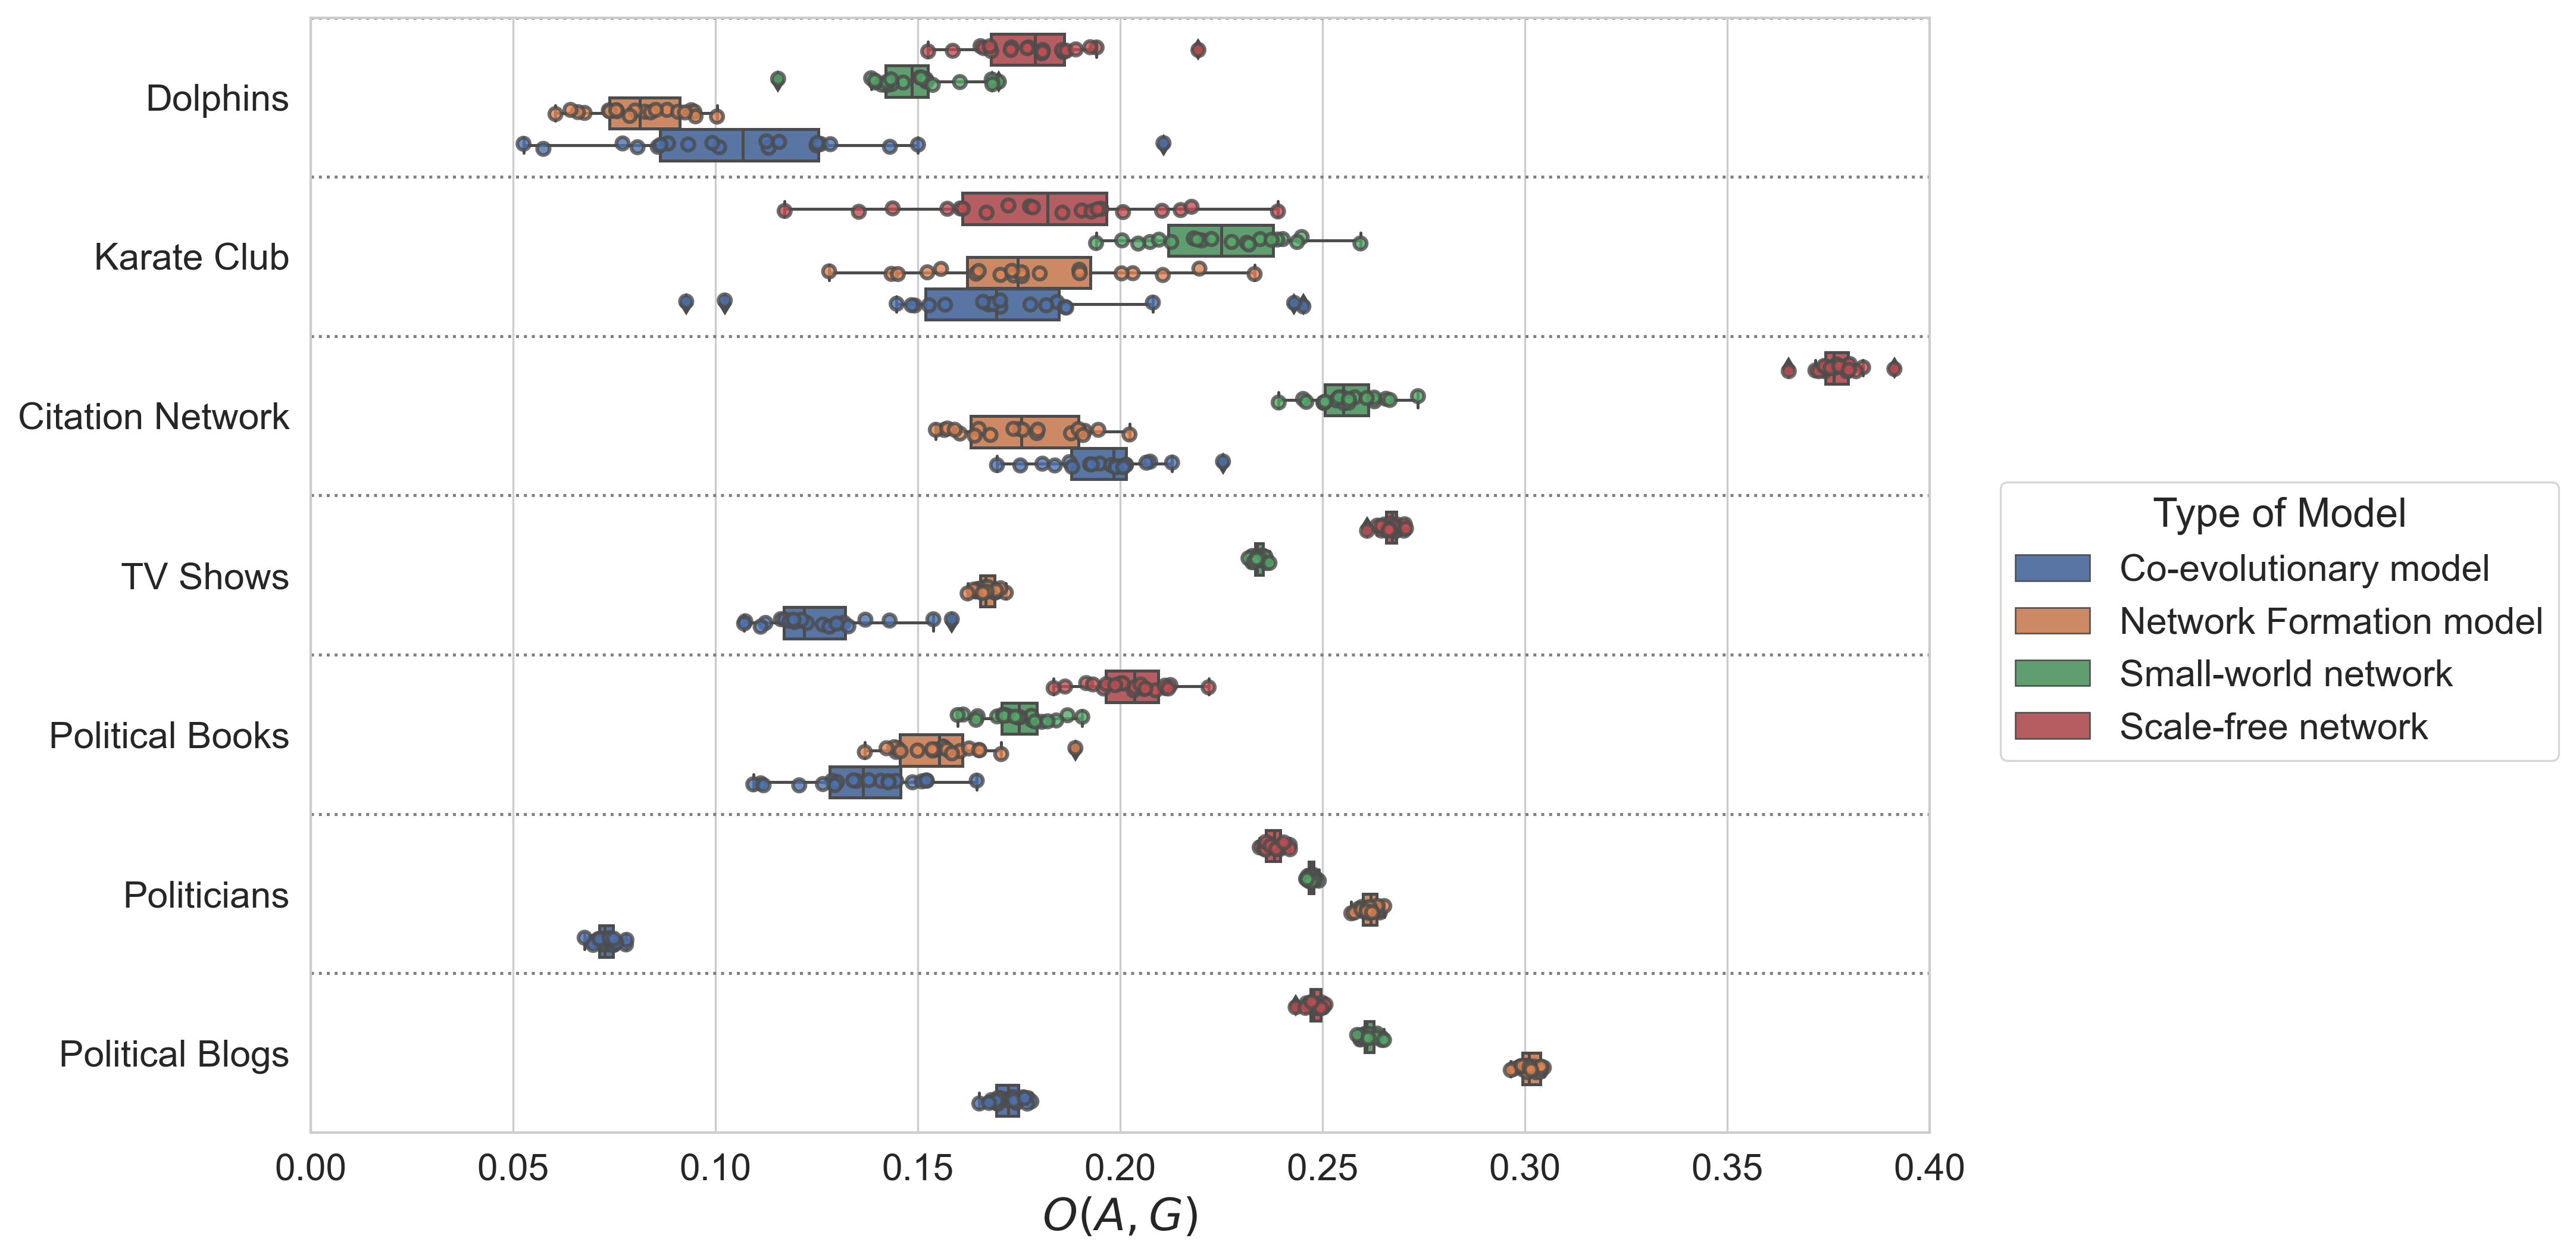
\includegraphics[width=.8\linewidth]{../plots/overall/Model_Evaluation.png}
  \caption{Difference in model performance. X-axis shows the mean difference between the generated network and actual networks, ($O(A, G)$). Y-axis shows the different empirical networks considered. Colors indicate whether the model includes or excludes opinion dynamics. Black lines indicate 95\% confidence intervals.}
  \label{fig:sfig1}
\end{figure}


\begin{table}[H]
\begin{center}
    
\begin{tabular}{ |p{3cm}||p{2cm}|p{2cm}|p{2cm}|p{2cm}|p{2cm}|}
    \hline
    \multicolumn{6}{|c|}{Table of best parameter values} \\
    \hline
    \bf{Network} & Randomness & Threshold & $\alpha$ & $\beta$ & $P(D)$\\
    \hline
    Dolphins   & 0.003    &0.531&   0.202&   0.095&   0.111\\
    Karate Club&   0.870  & 0.137   &0.282&   0.090&   0.911\\
    Citation Network   &0.060 & 0.655&  0.389&   0.493&   0.150\\
    TV Show & 0.038 & 0.157 & 0.349 & 0.093 & 0.751 \\
    Political Books &0.004 & 0.222&  0.075&   0.144&   0.508\\
    Politicians&   0.014  & 0.101 &0.050&   0.014&   0.229\\
    Political Blogs & 0.109  & 0.100   &0.246&   0.007&   0.249\\
    \hline
\end{tabular}
\end{center}
\caption{Table of best parameter values}
\end{table}

\begin{table}[H]
    \begin{center}
        
    \begin{tabular}{ |p{3cm}||p{1.5cm}|p{1.5cm}|p{1.5cm}|p{1.5cm}|p{1.5cm}|p{1.5cm}|}
        \hline
        \multicolumn{7}{|c|}{Table of network characteristics} \\
        \hline
        \bf{Network} & Nodes & Edges & $\mu$ & $\sigma$ & $C$ & $L_G$\\
        \hline
        Dolphins   & 62    &159&   5.129&   2.932 &   0.259 & 3.257\\
        Karate Club &34	&78	&4.588&	3.820&	0.571&	2.326\\
        Citation Network & 379 &	914	& 4.823	& 3.927 & 0.741 & 6.052 \\
        TV Shows & 3892 & 17262&8.871 & 12.557 & 0.374&6.324\\
        Political Books &105 &	441	& 8.400 &	5.449 &	0.488 &	3.015\\
        Politicians&  5908 &41729 & 14.126 & 20.096 &	0.385 & 4.628\\
        Political Blogs &	1222 & 16717 & 27.360 & 38.402 & 0.320 & 2.737\\
        \hline
    \end{tabular}
    \end{center}
    \caption{Table of network characteristics.}
    \end{table}

\subsection{Why is co-evolution a better explanation?}

Of particular interest is the political networks, as we know that these networks are likely to be highly opinionated. As the model performance shows, these are also the networks where the difference in performance between the network formation and the co-evolutionary model become most stark. Most notably, the difference in performance for the network of politicians and of political blogs is drastic. It is therefore worthwhile to consider why the co-evolutionary model fits these types of networks so much better than the network formation model.
One of the primary reasons for why the co-evolutionary model performs so much better on political social networks is that it enables the network to have multiple central hubs. By letting the threshold, B, be relatively low, the network balkanizes into different communities, exhibiting connected caveman properties (Watts, 1999). This is also in line with the fact that these two networks are the only networks considered, where threshold is the most important parameter. This suggests that the political networks are organized by clearly delineated communities. The balkanization obviously affects all the considered network characteristics considerably. Having low values of thresholds makes for networks with a much larger average path length than if all nodes were in one cluster.  As the communities become smaller in size, this affects the degree distribution as well. When the network is no longer organized around one central cluster, the resulting degree distribution will exhibit a shorter tail, as agents cannot connect to a large portion of the agents in the network. When a network is characterized by larger average path length and shorter tail degree distributions, the co-evolutionary model can outperform the model without opinion dynamics. Because of the co-evolutionary model’s ability to create multiple hubs, it can capture these phenomena well. In contrast, the network formation model only has one parameter, R. It has no way of reliably creating multiple clusters in the network, and therefore it fails when it encounters networks with clearly separated communities. The network formation model has to balance average path length and high clustering coefficient, as it can only vary how random new connections are, similar to small world networks (Watts \& Strogatz, 1998). The co-evolutionary model can change the size of different clusters by adjusting the confidence boundary and the tie-deletion parameter. 
This explanation seems to be in line with the importance of the different parameters for the model fit. A congruent point comes from considered the best parameters for the different political social networks. Most of them are characterized by very low confidence boundaries, very low amount of randomness, very low negative learning rate and moderate values for tie-deletion. As we’ve established, low confidence boundaries reflect that the political scene consists of different groups, that are locally very well connected, but doesn’t have much to do with each other. To achieve the high average clustering coefficients, the randomness must be low. For the network to not just become two clusters, negative learning rate must be low, so that opinions do not cluster around 1 and -1. Finally, to ensure that there is still some global connectivity between the different clusters, tie deletion is not high enough to limit the network to only have one or two informational highways. 

In conclusion, the agent-based model fitting and model comparison suggests two important notions. The first notion is that triadic closure alone seems to be able to generate many of the characteristic patterns of social network. This echoes previous findings concluding the same (Ilany \& Akçay, 2016; Jackson \& Rogers, 2004, 2007). The second notion is that when opinions are central to the social networks, including opinion dynamics makes for a markedly better model of why social networks are like they are. 
This second notion points to the fact that the effects of network and opinion dynamics are largely interdependent. We have seen that opinion dynamics can drastically alter the dynamics of networks. We now turn to the other side of this interplay by considering how network dynamics can change opinions.

\section{Results}

\subsection{Alpha, beta, threshold, tie-deletion and chaotic systems}

\subsection{Correlations}

\section{Discussion}

\subsection{Reiterating previous literature}

\subsection{Tie-deletion facilitates cooperation}

\subsection{The effect of initial opinions}

\subsection{Distance in opinion and network space}

\section{Short comings and future work}

\subsection{Accurate perceptions of opinions}

\subsection{Social influence exclusively}

\section{A broader perspective}

\section{Conclusion}

\bibliographystyle{apacite}

\bibliography{References}

\end{document}